\documentclass{beamer}
\usepackage[utf8]{inputenc}

\usetheme{Madrid}
\usecolortheme{default}
\usepackage{amsmath,amssymb,amsfonts,amsthm}
\usepackage{txfonts}
\usepackage{tkz-euclide}
\usepackage{listings}
\usepackage{adjustbox}
\usepackage{array}
\usepackage{tabularx}
\usepackage{gvv}
\usepackage{multicol}   % <-- Add this

\usepackage{lmodern}
\usepackage{circuitikz}
\usepackage{tikz}
\usepackage{graphicx}
\usepackage{mathtools}
\setbeamertemplate{page number in head/foot}[totalframenumber]

\usepackage{tcolorbox}
\tcbuselibrary{minted,breakable,xparse,skins}



\definecolor{bg}{gray}{0.95}
\DeclareTCBListing{mintedbox}{O{}m!O{}}{%
  breakable=true,
  listing engine=minted,
  listing only,
  minted language=#2,
  minted style=default,
  minted options={%
    linenos,
    gobble=0,
    breaklines=true,
    breakafter=,,
    fontsize=\small,
    numbersep=8pt,
    #1},
  boxsep=0pt,
  left skip=0pt,
  right skip=0pt,
  left=25pt,
  right=0pt,
  top=3pt,
  bottom=3pt,
  arc=5pt,
  leftrule=0pt,
  rightrule=0pt,
  bottomrule=2pt,
  toprule=2pt,
  colback=bg,
  colframe=orange!70,
  enhanced,
  overlay={%
    \begin{tcbclipinterior}
    \fill[orange!20!white] (frame.south west) rectangle ([xshift=20pt]frame.north west);
    \end{tcbclipinterior}},
  #3,
}
\lstset{
    language=C,
    basicstyle=\ttfamily\small,
    keywordstyle=\color{blue},
    stringstyle=\color{orange},
    commentstyle=\color{green!60!black},
    numbers=left,
    numberstyle=\tiny\color{gray},
    breaklines=true,
    showstringspaces=false,
}


\title 
{4.13.79}
\date{October 3, 2025}


\author 
{Dhanush Kumar A - AI25BTECH11010}



\begin{document}
\frame{\titlepage}
\begin{frame}{Question}
In $\mathbb{R}^3$, let $L$ be a straight line passing through the origin. Suppose that all the points on $L$ are at a constant distance from two planes:$
P_1 : x+2y-z+1=0, 
P_2 : 2x-y+z-1=0.$
Let $M$ be the locus of the feet of the perpendicular drawn from the points on $L$ to the plane $P_1$. Which of the following points lie(s) on $M$?


		\begin{multicols}{2}
			\begin{enumerate}


\item $\myvec{0\\ -\tfrac{5}{6}\\ -\tfrac{2}{3}}$
\item $\myvec{-\tfrac{1}{6}\\ -\tfrac{1}{3}\\ \tfrac{1}{6}}$
\item $\myvec{-\tfrac{5}{6}\\ 0\\ \tfrac{2}{3}}$
\item $\myvec{-\tfrac{1}{3}\\ 0\\ \tfrac{2}{3}}$
	\end{enumerate}
\end{multicols}

\end{frame}
\begin{frame}{Solution}
Step 1: Direction vector of $L$
\begin{align}
\vec{r}_L(t) &= t \vec{D}, \\
\vec{n}_1 &= \myvec{1\\2\\-1}, & \vec{n}_2 &= \myvec{2\\-1\\1}, \\
\vec{n}_1^T \vec{D} &= 0, & \vec{n}_2^T \vec{D} &= 0.
\end{align}

\begin{align}
	\myvec{\vec{n}_1 && \vec{n}_2}^T \vec{D} &= 0, \\
\vec{D} &= \myvec{1\\-3\\-5}, \\
\vec{r}_L(t) &= t \vec{D}.
\end{align}
\end{frame}
\begin{frame}{Solution}

Step 2: Foot of perpendicular to $P_1$
\begin{align}
\vec{r}_M &= \vec{r}_L(t) + \lambda \vec{n}_1, \\
&= t \vec{D} + \lambda \myvec{1\\2\\-1}, \\
\vec{n}_1^T \vec{r}_M + 1 &= 0, \\
\vec{n}_1^T \bigl( t \vec{D} + \lambda \myvec{1\\2\\-1} \bigr) + 1 &= 0, \\
\vec{n}_1^T \vec{r}_L(t) &= 1\cdot t + 2(-3t) + (-1)(-5t) = 0, \\
\vec{n}_1^T \vec{n}_1 &= 1^2 + 2^2 + (-1)^2 = 6, \\
\end{align}
\end{frame}

\begin{frame}{Solution}
\begin{align}
6 \lambda + 1 &= 0 \;\Rightarrow\; \lambda = -\tfrac{1}{6}, \\
\vec{r}_M &= t \vec{D} - \tfrac{1}{6} \vcenter{\hbox{\myvec{1\\2\\-1}}}, \\
\vec{r}_M &= \vcenter{\hbox{\myvec{t-\tfrac{1}{6}\\ -3t-\tfrac{1}{3}\\ -5t+\tfrac{1}{6}}}}.
\end{align}

\text{Step 3: Checking the options}
\begin{align}
\text{Option (a):} \quad 
\vcenter{\hbox{\myvec{0\\ -\tfrac{5}{6}\\ -\tfrac{2}{3}}}} 
&= \vcenter{\hbox{\myvec{t-\tfrac{1}{6}\\ -3t-\tfrac{1}{3}\\ -5t+\tfrac{1}{6}}}} 
\;\Rightarrow\; t = \tfrac{1}{6}, \quad \text{lies on $M$},\\[1mm]
\text{Option (b):} \quad
\vcenter{\hbox{\myvec{-\tfrac{1}{6}\\ -\tfrac{1}{3}\\ \tfrac{1}{6}}}} 
&= \vcenter{\hbox{\myvec{t-\tfrac{1}{6}\\ -3t-\tfrac{1}{3}\\ -5t+\tfrac{1}{6}}}} 
\;\Rightarrow\; t = 0, \quad \text{lies on $M$}.
\end{align}
\end{frame}

\begin{frame}{Solution}
\begin{align}
\text{Option (c):} \quad
\vcenter{\hbox{\myvec{-\tfrac{5}{6}\\ 0\\ \tfrac{2}{3}}}} 
&= \vcenter{\hbox{\myvec{t-\tfrac{1}{6}\\ -3t-\tfrac{1}{3}\\ -5t+\tfrac{1}{6}}}} 
\;\Rightarrow\; t=-\tfrac{2}{3}, \quad y = \tfrac{5}{3} \neq 0, \quad \text{does not lie on $M$},\\[1mm]
\text{Option (d):} \quad
\vcenter{\hbox{\myvec{-\tfrac{1}{3}\\ 0\\ \tfrac{2}{3}}}} 
&= \vcenter{\hbox{\myvec{t-\tfrac{1}{6}\\ -3t-\tfrac{1}{3}\\ -5t+\tfrac{1}{6}}}} 
\;\Rightarrow\; t=-\tfrac{1}{6}, \quad y = \tfrac{1}{6} \neq 0, \quad \text{does not lie on $M$}.
\end{align}
\end{frame}

\begin{frame}{Solution}
\begin{align}
\vec{r}_M &= \vcenter{\hbox{\myvec{t-\tfrac{1}{6}\\ -3t-\tfrac{1}{3}\\ -5t+\tfrac{1}{6}}}}, \quad t \in \mathbb{R}, \\
\text{Points on $M$} &= \vcenter{\hbox{\myvec{0\\ -\tfrac{5}{6}\\ -\tfrac{2}{3}}}}, \;\; 
\vcenter{\hbox{\myvec{-\tfrac{1}{6}\\ -\tfrac{1}{3}\\ \tfrac{1}{6}}}}.
\end{align}
\end{frame}

\begin{frame}{Plot}
    \centering
    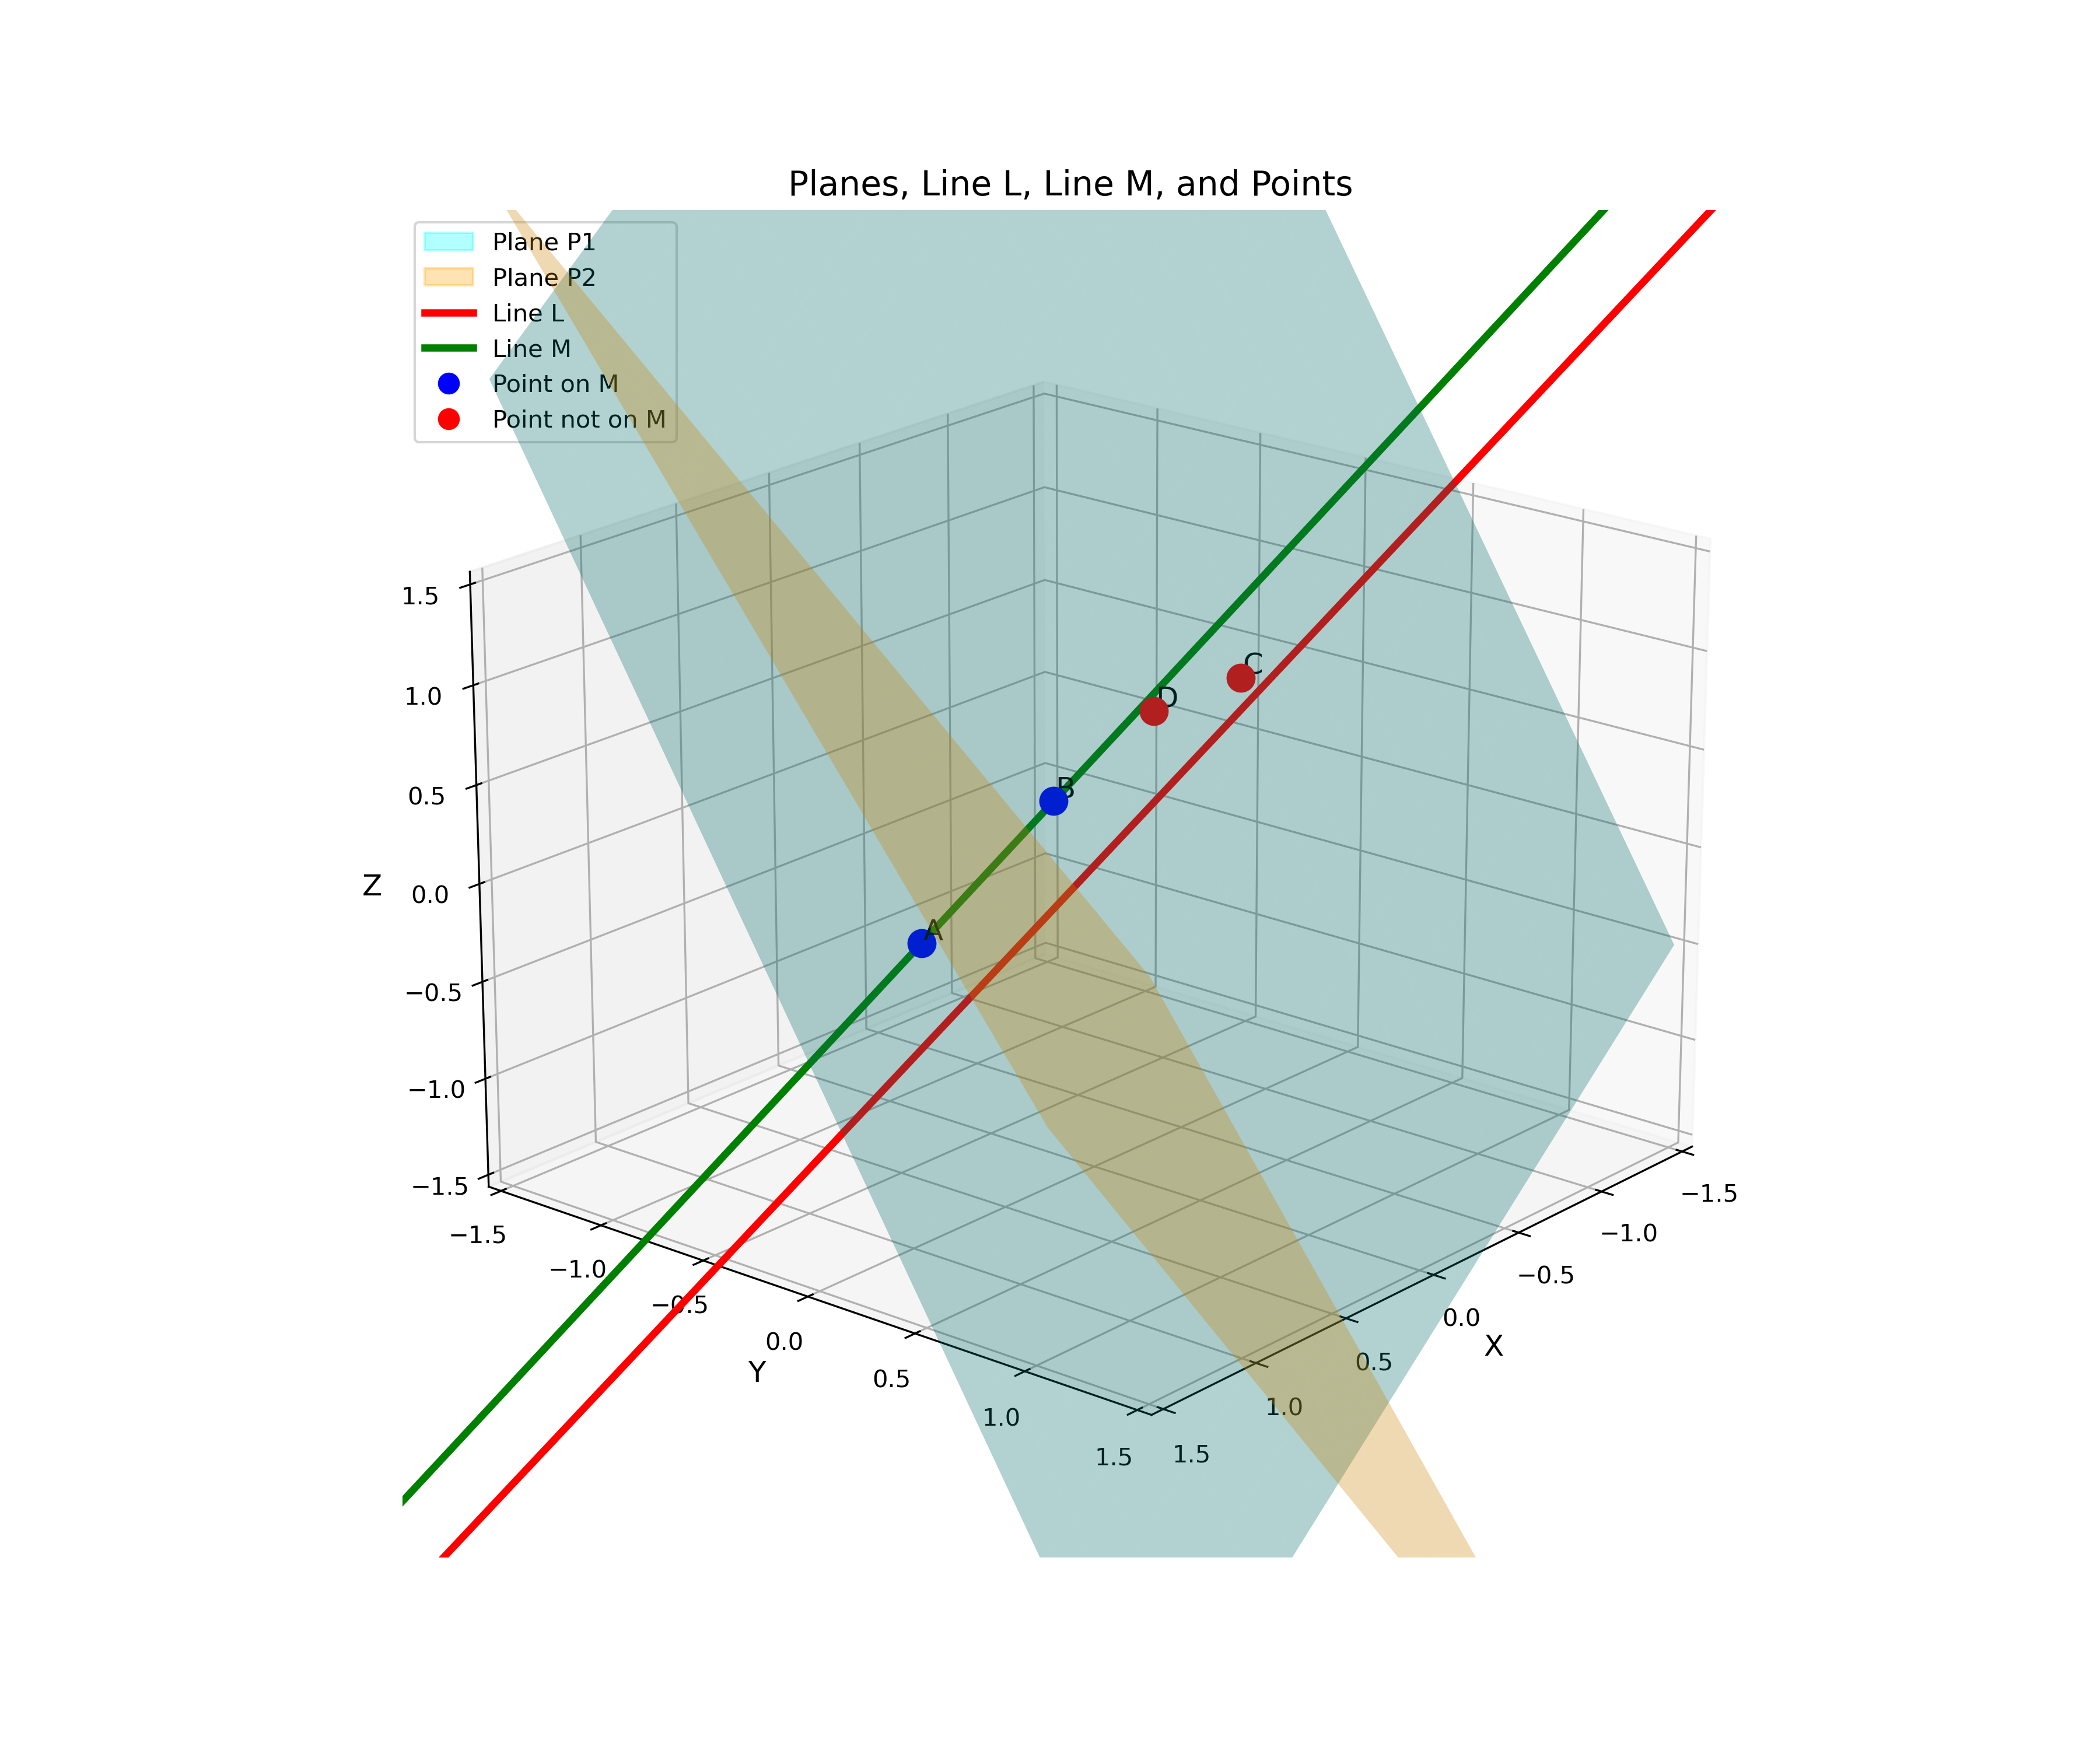
\includegraphics[width=\columnwidth, height=0.8\textheight, keepaspectratio]{../figs/planes_lines_points.png}     
\end{frame}


\begin{frame}[fragile]                            
\frametitle{Python code - To check the points }                
\begin{lstlisting}

import numpy as np
import matplotlib.pyplot as plt
from mpl_toolkits.mplot3d import Axes3D
import os
from matplotlib.lines import Line2D
import matplotlib.patches as mpatches

# ---------- Plane normals ----------
n1 = np.array([1, 2, -1], dtype=float)
n2 = np.array([2, -1, 1], dtype=float)

# ---------- Direction vector of L ----------
d = np.cross(n1, n2)
print("Direction vector of L:", d)
\end{lstlisting}
\end{frame}
\begin{frame}[fragile]                            
\frametitle{Python code - To check the points }                
\begin{lstlisting}

# ---------- Line definitions ----------
def rL(t):
    return t * d

def rM(t):
    lam = -1 / np.dot(n1, n1)
    return t*d + lam*n1

# ---------- Option points ----------
A = np.array([0, -5/6, -2/3], dtype=float)
B = np.array([-1/6, -1/3, 1/6], dtype=float)
C = np.array([-5/6, 0, 2/3], dtype=float)
D = np.array([-1/3, 0, 2/3], dtype=float)
points = {"A": A, "B": B, "C": C, "D": D}
\end{lstlisting}
\end{frame}
\begin{frame}[fragile]                            
\frametitle{Python code - To check the points }                
\begin{lstlisting}

# ---------- Check if point lies on M ----------
def is_on_M(P, d, n1, tol=1e-6):
    lam = -1 / np.dot(n1, n1)
    P_shift = P - lam * n1
    t = np.dot(d, P_shift) / np.dot(d, d)
    distance = np.linalg.norm(P_shift - t*d)
    return distance < tol

# ---------- Check points ----------
for label, P in points.items():
    if is_on_M(P, d, n1):
        print(f"Point {label} lies on line M")
    else:
        print(f"Point {label} does NOT lie on line M")



\end{lstlisting}
\end{frame}

\begin{frame}[fragile]                            
\frametitle{Python code - Plotting the Plane}                
\begin{lstlisting}
# ---------- Plot ----------
fig = plt.figure(figsize=(12, 10))
ax = fig.add_subplot(111, projection='3d')

# Planes
xx, yy = np.meshgrid(np.linspace(-1.5, 1.5, 20), np.linspace(-1.5, 1.5, 20))
zz1 = 1 - xx - 2*yy
zz2 = -1 + 2*xx - yy
ax.plot_surface(xx, yy, zz1, alpha=0.3, color='cyan')
ax.plot_surface(xx, yy, zz2, alpha=0.3, color='orange')

# Line L
t_vals = np.linspace(-1.5, 1.5, 200)
L_points = np.array([rL(t) for t in t_vals])
ax.plot(L_points[:,0], L_points[:,1], L_points[:,2], 'r', linewidth=3, label='Line L')
\end{lstlisting}
\end{frame}

\begin{frame}[fragile]                            
\frametitle{Python code - Plotting the Plane}                
\begin{lstlisting}

# Line M
M_points = np.array([rM(t) for t in t_vals])
ax.plot(M_points[:,0], M_points[:,1], M_points[:,2], 'g', linewidth=3, label='Line M')

# Plot points with labels
for label, P in points.items():
    color = 'blue' if is_on_M(P, d, n1) else 'red'
    ax.scatter(P[0], P[1], P[2], s=120, c=color)
    ax.text(P[0]+0.05, P[1]+0.05, P[2]+0.05, label, fontsize=12)
\end{lstlisting}
\end{frame}

\begin{frame}[fragile]                            
\frametitle{Python code - Plotting the Plane}                
\begin{lstlisting}

# ---------- Create legend manually ----------
legend_elements = [
    mpatches.Patch(facecolor='cyan', edgecolor='cyan', alpha=0.3, label='Plane P1'),
    mpatches.Patch(facecolor='orange', edgecolor='orange', alpha=0.3, label='Plane P2'),
    Line2D([0], [0], color='r', lw=3, label='Line L'),
    Line2D([0], [0], color='g', lw=3, label='Line M'),
    Line2D([0], [0], marker='o', color='w', markerfacecolor='blue', markersize=10, label='Point on M'),
    Line2D([0], [0], marker='o', color='w', markerfacecolor='red', markersize=10, label='Point not on M')
]
ax.legend(handles=legend_elements, loc='upper left', fontsize=10)
\end{lstlisting}
\end{frame}

\begin{frame}[fragile]                            
\frametitle{Python code - Plotting the Plane}                
\begin{lstlisting}

# Axis labels
ax.set_xlabel('X', fontsize=12)
ax.set_ylabel('Y', fontsize=12)
ax.set_zlabel('Z', fontsize=12)
ax.set_title("Planes, Line L, Line M, and Points ", fontsize=14)

# Axis limits and grid
ax.set_xlim(-1.5, 1.5)
ax.set_ylim(-1.5, 1.5)
ax.set_zlim(-1.5, 1.5)
ax.grid(True)
\end{lstlisting}
\end{frame}

\begin{frame}[fragile]                            
\frametitle{Python code - Plotting the Plane}                
\begin{lstlisting}

# Viewing angle
ax.view_init(elev=20, azim=40)

# Ensure directory exists and save figure
os.makedirs("figs", exist_ok=True)
fig_path = os.path.join("../figs", "planes_lines_points.png")
plt.savefig(fig_path, dpi=300)
print(f"Figure saved at: {fig_path}")

plt.show()
\end{lstlisting}

\end{frame}
\begin{frame}{Plot-Using  Python}
    \centering
    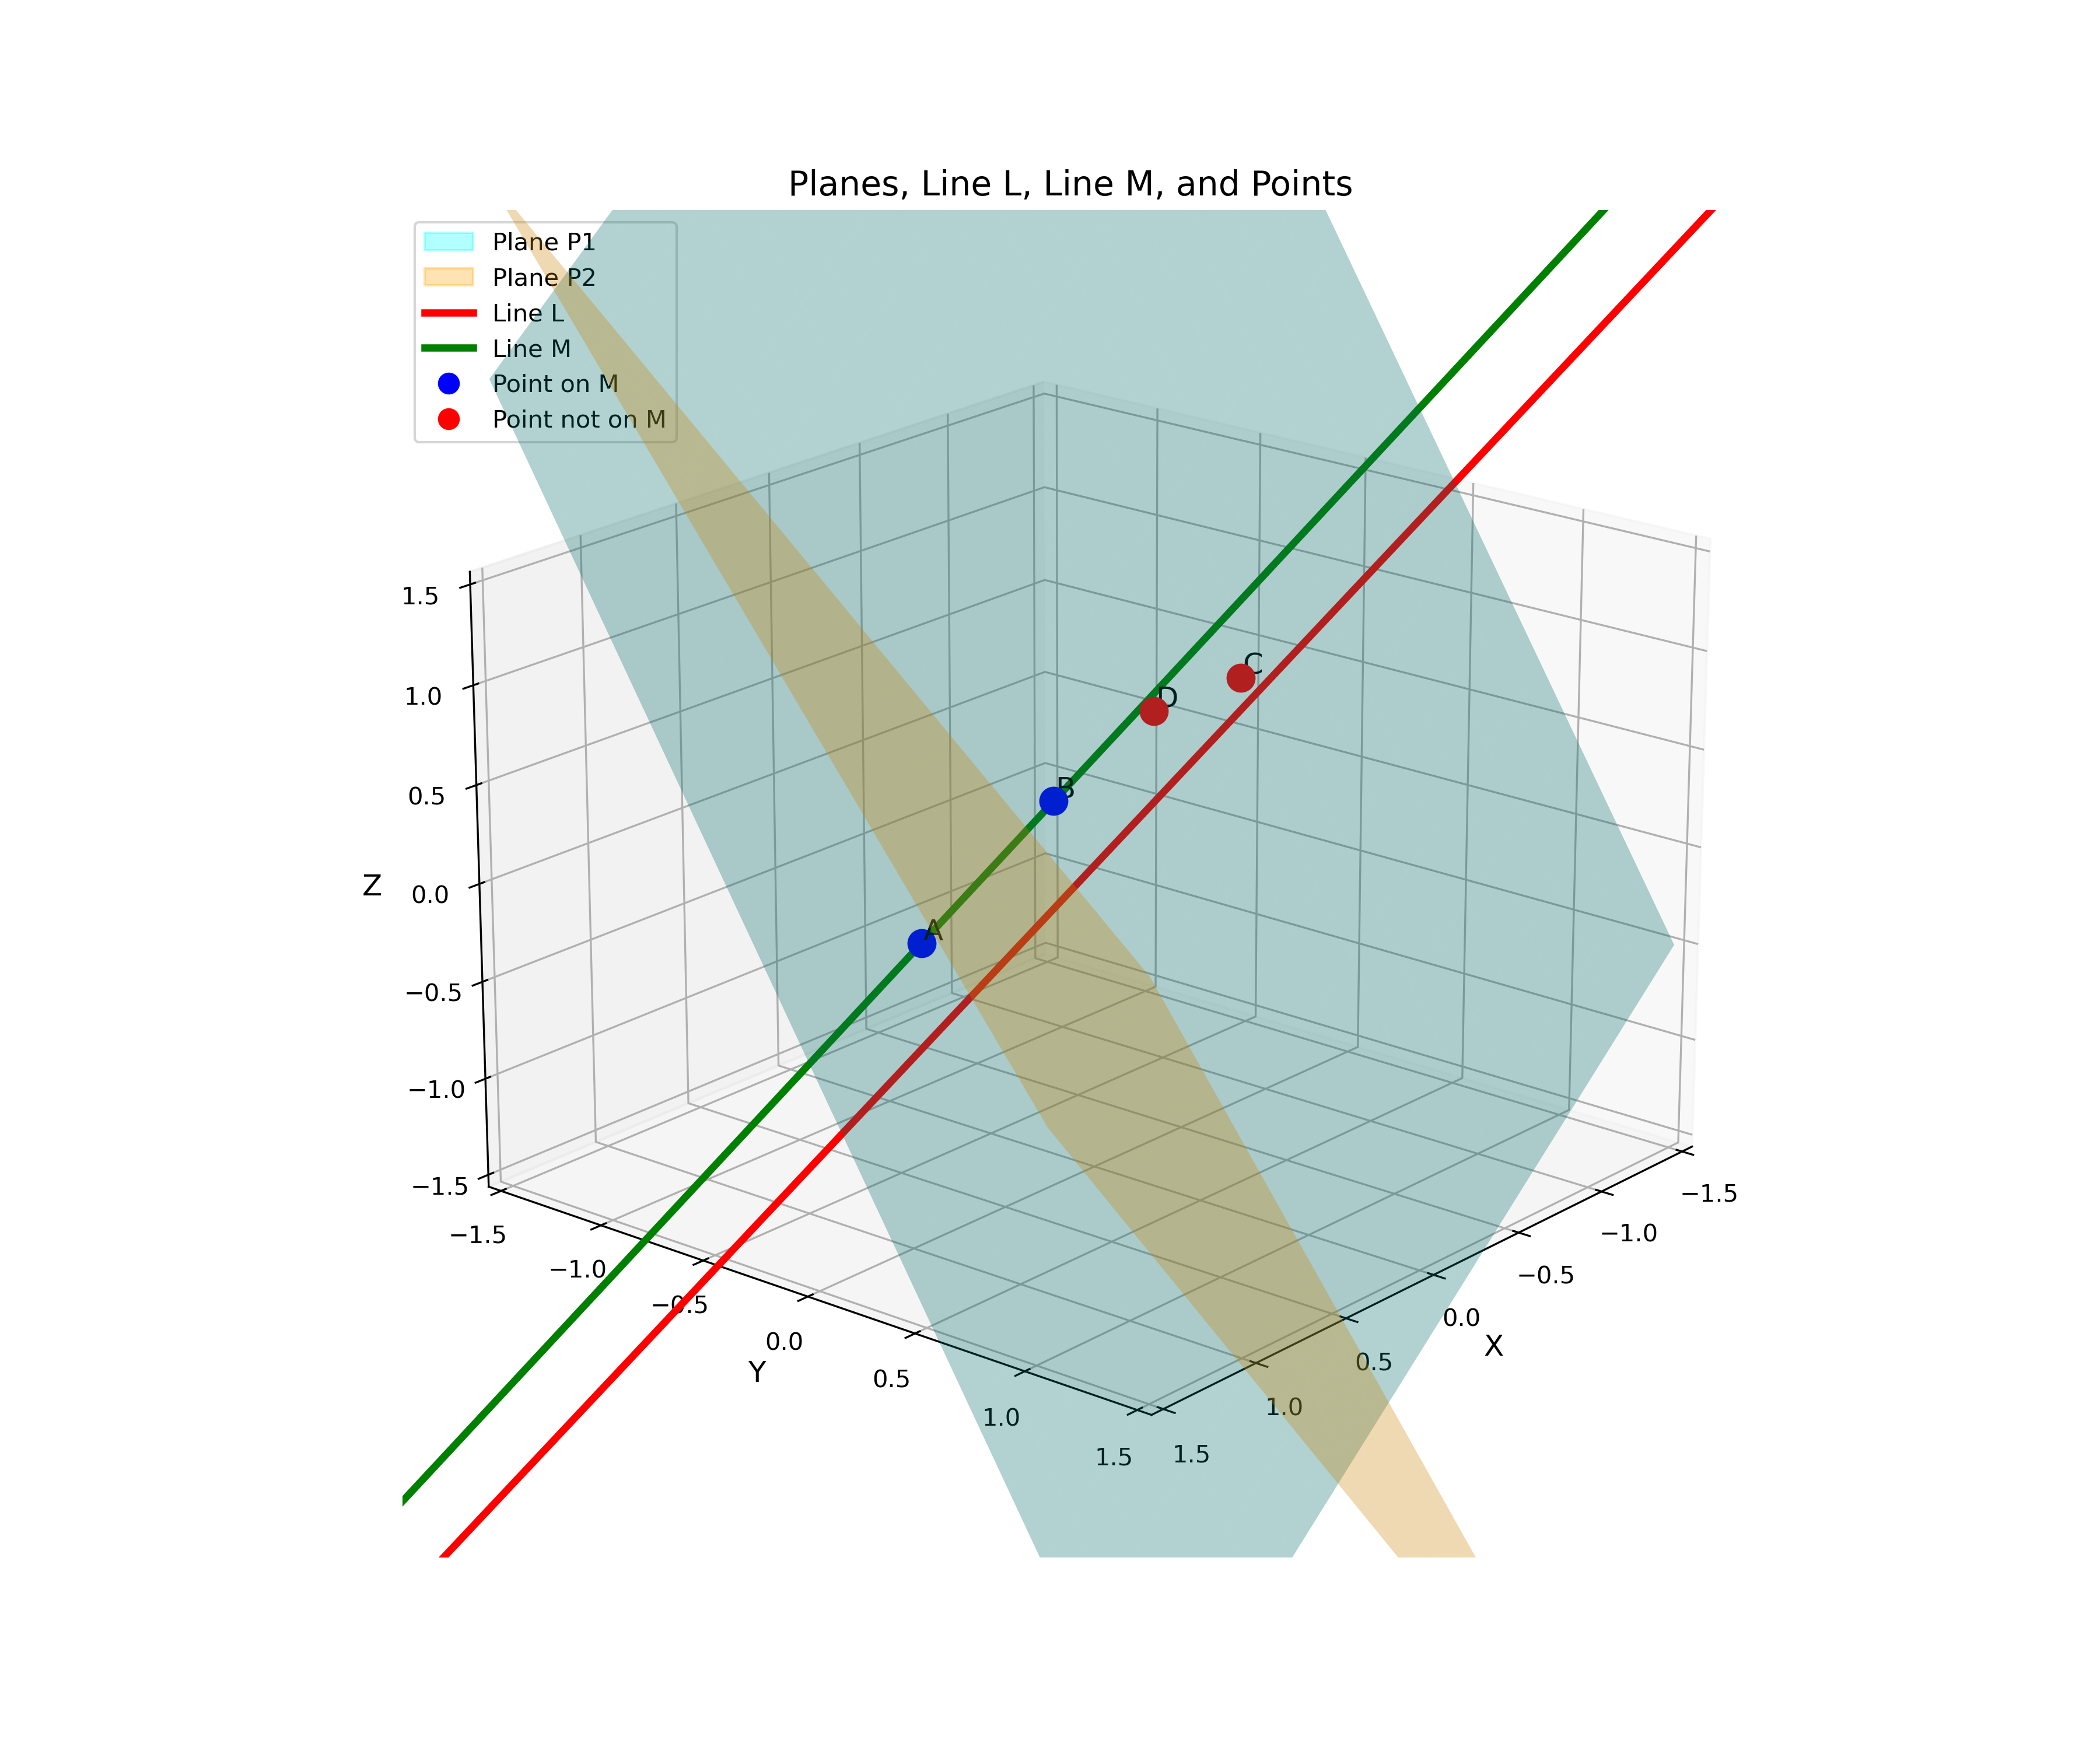
\includegraphics[width=\columnwidth, height=0.8\textheight, keepaspectratio]{../figs/planes_lines_points.png}     

\end{frame}

\begin{frame}[fragile]                            
\frametitle{C code - Solving}                
\begin{lstlisting}
#include <stdio.h>
#include <stdlib.h>
#include <math.h>
#include "/home/dhanush-kumar-a/ee1030-2025/ai25btech11010/matgeo/4.13.79/codes/libs/matfun.h"

// Compute locus M and check candidate points
void compute_locus_check(
    double **n1, double **n2, double d1,
    int nt, double *t_values,
    double **Qs,       // 3 x nt
    double *d_vec,     // 3x1 line direction
    double **pts, int *truths // 4 candidate points
){
    // Step 1: Compute line direction d = n1 x n2
    d_vec[0] = n1[1][0]*n2[2][0] - n1[2][0]*n2[1][0];
    d_vec[1] = n1[2][0]*n2[0][0] - n1[0][0]*n2[2][0];
    d_vec[2] = n1[0][0]*n2[1][0] - n1[1][0]*n2[0][0];
\end{lstlisting}
\end{frame}
\begin{frame}[fragile]                            
\frametitle{C code - Solving}                
\begin{lstlisting}


    // Normalize d_vec
    double norm_d = sqrt(d_vec[0]*d_vec[0] + d_vec[1]*d_vec[1] + d_vec[2]*d_vec[2]);
    for(int i=0;i<3;i++) d_vec[i] /= norm_d;

    // Step 2: Compute locus points Qs for each t
    for(int k=0;k<nt;k++){
        double t = t_values[k];
        double **P = createMat(3,1);
        for(int i=0;i<3;i++) P[i][0] = t * d_vec[i];

        // Foot of perpendicular to plane P1: Q = P - lambda*n1
        double lam = (Matdot(n1,P,3) + d1) / Matdot(n1,n1,3); // note +d1 since plane: n^T x + d = 0
        double **Q = Matsub(P, Matscale(n1,3,1,lam), 3,1);
\end{lstlisting}
\end{frame}
\begin{frame}[fragile]                            
\frametitle{C code - Solving}                
\begin{lstlisting}

        // Save Q to Qs
        for(int i=0;i<3;i++) Qs[i][k] = Q[i][0];

        // Free temporary matrices
        for(int i=0;i<3;i++) free(P[i]);
        free(P);
        for(int i=0;i<3;i++) free(Q[i]);
        free(Q);
    }

    // Step 3: Check candidate points a,b,c,d
    for(int p=0;p<4;p++){
        double *pt = pts[p];
\end{lstlisting}
\end{frame}
\begin{frame}[fragile]                            
\frametitle{C code - Solving}                
\begin{lstlisting}

        // Solve t and lambda from rM = t*d + lambda*n1
        double t_num = pt[0]*d_vec[0] + pt[1]*d_vec[1] + pt[2]*d_vec[2];
        double t_den = d_vec[0]*d_vec[0] + d_vec[1]*d_vec[1] + d_vec[2]*d_vec[2];
        double t = t_num / t_den;

        double lambda_num = n1[0][0]*(pt[0]-t*d_vec[0]) +
                            n1[1][0]*(pt[1]-t*d_vec[1]) +
                            n1[2][0]*(pt[2]-t*d_vec[2]);
        double lambda_den = Matdot(n1,n1,3);
        double lam = lambda_num / lambda_den;
\end{lstlisting}
\end{frame}
\begin{frame}[fragile]                            
\frametitle{C code - Solving}                
\begin{lstlisting}

        // Projected point on M
        double xM = t*d_vec[0] + lam*n1[0][0];
        double yM = t*d_vec[1] + lam*n1[1][0];
        double zM = t*d_vec[2] + lam*n1[2][0];

        // Check if close to original point
        double eps = 1e-6;
        truths[p] = (fabs(xM-pt[0])<eps && fabs(yM-pt[1])<eps && fabs(zM-pt[2])<eps) ? 1 : 0;
    }
}


\end{lstlisting}
\end{frame}

	
\begin{frame}[fragile]                              
	\frametitle{Python code -Ploting the plane using c function} 
	\begin{lstlisting}
import ctypes
import numpy as np
import matplotlib.pyplot as plt
from mpl_toolkits.mplot3d import Axes3D
import os
from matplotlib.lines import Line2D
import matplotlib.patches as mpatches

# Load the shared library
lib = ctypes.CDLL("./main.so")  # make sure to compile the C file as liblocus.so
\end{lstlisting}
\end{frame}

	
\begin{frame}[fragile]                              
	\frametitle{Python code -Ploting the plane using c function} 
	\begin{lstlisting}

# Define ctypes argument types
lib.compute_locus_check.argtypes = [
    ctypes.POINTER(ctypes.POINTER(ctypes.c_double)),  # n1
    ctypes.POINTER(ctypes.POINTER(ctypes.c_double)),  # n2
    ctypes.c_double,                                  # d1
    ctypes.c_int,                                     # nt
    np.ctypeslib.ndpointer(dtype=np.float64, ndim=1),# t_values
    ctypes.POINTER(ctypes.POINTER(ctypes.c_double)),  # Qs (3 x nt)
    np.ctypeslib.ndpointer(dtype=np.float64, ndim=1),# d_vec (3)
    ctypes.POINTER(ctypes.POINTER(ctypes.c_double)),  # pts (4x3)
    np.ctypeslib.ndpointer(dtype=np.int32, ndim=1)   # truths (4)
]
\end{lstlisting}
\end{frame}

	
\begin{frame}[fragile]                              
	\frametitle{Python code -Ploting the plane using c function} 
	\begin{lstlisting}

# ---------- Input data ----------
n1 = np.array([1.0, 2.0, -1.0], dtype=np.float64)
n2 = np.array([2.0, -1.0, 1.0], dtype=np.float64)
d1 = 1.0

# Candidate points a,b,c,d
pts_values = np.array([
    [0, -5/6, -2/3],
    [-1/6, -1/3, 1/6],
    [-5/6, 0, 2/3],
    [-1/3, 0, 2/3]
], dtype=np.float64)

# Number of t values along L
nt = 200
t_values = np.linspace(-1.5, 1.5, nt, dtype=np.float64)
\end{lstlisting}
\end{frame}

	
\begin{frame}[fragile]                              
	\frametitle{Python code -Ploting the plane using c function} 
	\begin{lstlisting}

# Allocate memory for Qs (3 x nt)
Qs = (ctypes.POINTER(ctypes.c_double) * 3)()
for i in range(3):
    Qs[i] = (ctypes.c_double * nt)()

# Allocate memory for points array
pts = (ctypes.POINTER(ctypes.c_double) * 4)()
for i in range(4):
    pts[i] = (ctypes.c_double * 3)(*pts_values[i])

# Allocate memory for d_vec and truths
d_vec = np.zeros(3, dtype=np.float64)
truths = np.zeros(4, dtype=np.int32)
\end{lstlisting}
\end{frame}

	
\begin{frame}[fragile]                              
	\frametitle{Python code -Ploting the plane using c function} 
	\begin{lstlisting}

# Convert n1, n2 to ctypes pointers
n1_ct = (ctypes.POINTER(ctypes.c_double) * 3)()
n2_ct = (ctypes.POINTER(ctypes.c_double) * 3)()
for i in range(3):
    n1_ct[i] = ctypes.pointer(ctypes.c_double(n1[i]))
    n2_ct[i] = ctypes.pointer(ctypes.c_double(n2[i]))

# Call the C function
lib.compute_locus_check(n1_ct, n2_ct, d1, nt, t_values, Qs, d_vec, pts, truths)

# ---------- Print results ----------
for i, label in enumerate(['A','B','C','D']):
    print(f"Point {label} lies on M? {'Yes' if truths[i]==1 else 'No'}")
print("Direction vector of line L:", d_vec)
\end{lstlisting}
\end{frame}

	
\begin{frame}[fragile]                              
	\frametitle{Python code -Ploting the plane using c function} 
	\begin{lstlisting}

# ---------- Plot ----------
fig = plt.figure(figsize=(12,10))
ax = fig.add_subplot(111, projection='3d')

# Planes
xx, yy = np.meshgrid(np.linspace(-1.5,1.5,20), np.linspace(-1.5,1.5,20))
zz1 = (-d1 - n1[0]*xx - n1[1]*yy)/n1[2]
zz2 = (-(-1) - n2[0]*xx - n2[1]*yy)/n2[2]
ax.plot_surface(xx, yy, zz1, alpha=0.3, color='cyan')
ax.plot_surface(xx, yy, zz2, alpha=0.3, color='orange')

# Line L
t_vals = np.linspace(-1.5,1.5,200)
L_points = np.array([t*d_vec for t in t_vals])
ax.plot(L_points[:,0], L_points[:,1], L_points[:,2], 'r', linewidth=3, label='Line L')
\end{lstlisting}
\end{frame}

	
\begin{frame}[fragile]                              
	\frametitle{Python code -Ploting the plane using c function} 
	\begin{lstlisting}

# Line M (from Qs)
M_points = np.array([[Qs[i][k] for k in range(nt)] for i in range(3)]).T
ax.plot(M_points[:,0], M_points[:,1], M_points[:,2], 'g', linewidth=3, label='Line M')

# Plot candidate points
for i, label in enumerate(['A','B','C','D']):
    color = 'blue' if truths[i]==1 else 'red'
    P = pts_values[i]
    ax.scatter(P[0], P[1], P[2], s=120, c=color)
    ax.text(P[0]+0.05, P[1]+0.05, P[2]+0.05, label, fontsize=12)
\end{lstlisting}
\end{frame}

	
\begin{frame}[fragile]                              
	\frametitle{Python code -Ploting the plane using c function} 
	\begin{lstlisting}

# Legend
legend_elements = [
    mpatches.Patch(facecolor='cyan', alpha=0.3, label='Plane P1'),
    mpatches.Patch(facecolor='orange', alpha=0.3, label='Plane P2'),
    Line2D([0],[0], color='r', lw=3, label='Line L'),
    Line2D([0],[0], color='g', lw=3, label='Line M'),
    Line2D([0],[0], marker='o', color='w', markerfacecolor='blue', markersize=10, label='Point on M'),
    Line2D([0],[0], marker='o', color='w', markerfacecolor='red', markersize=10, label='Point not on M')
]
ax.legend(handles=legend_elements)
\end{lstlisting}
\end{frame}

	
\begin{frame}[fragile]                              
	\frametitle{Python code -Ploting the plane using c function} 
	\begin{lstlisting}

ax.set_xlabel('X'); ax.set_ylabel('Y'); ax.set_zlabel('Z')
ax.set_title("Planes, Line L, Line M, and Points")
ax.set_xlim(-1.5,1.5); ax.set_ylim(-1.5,1.5); ax.set_zlim(-1.5,1.5)
ax.view_init(elev=20, azim=40)

plt.savefig("../figs/planes_lines_points_ctypes.png", dpi=300)
plt.show()


\end{lstlisting}                               
\end{frame}

\begin{frame}{Plot-Using  Python and C}
    \centering
    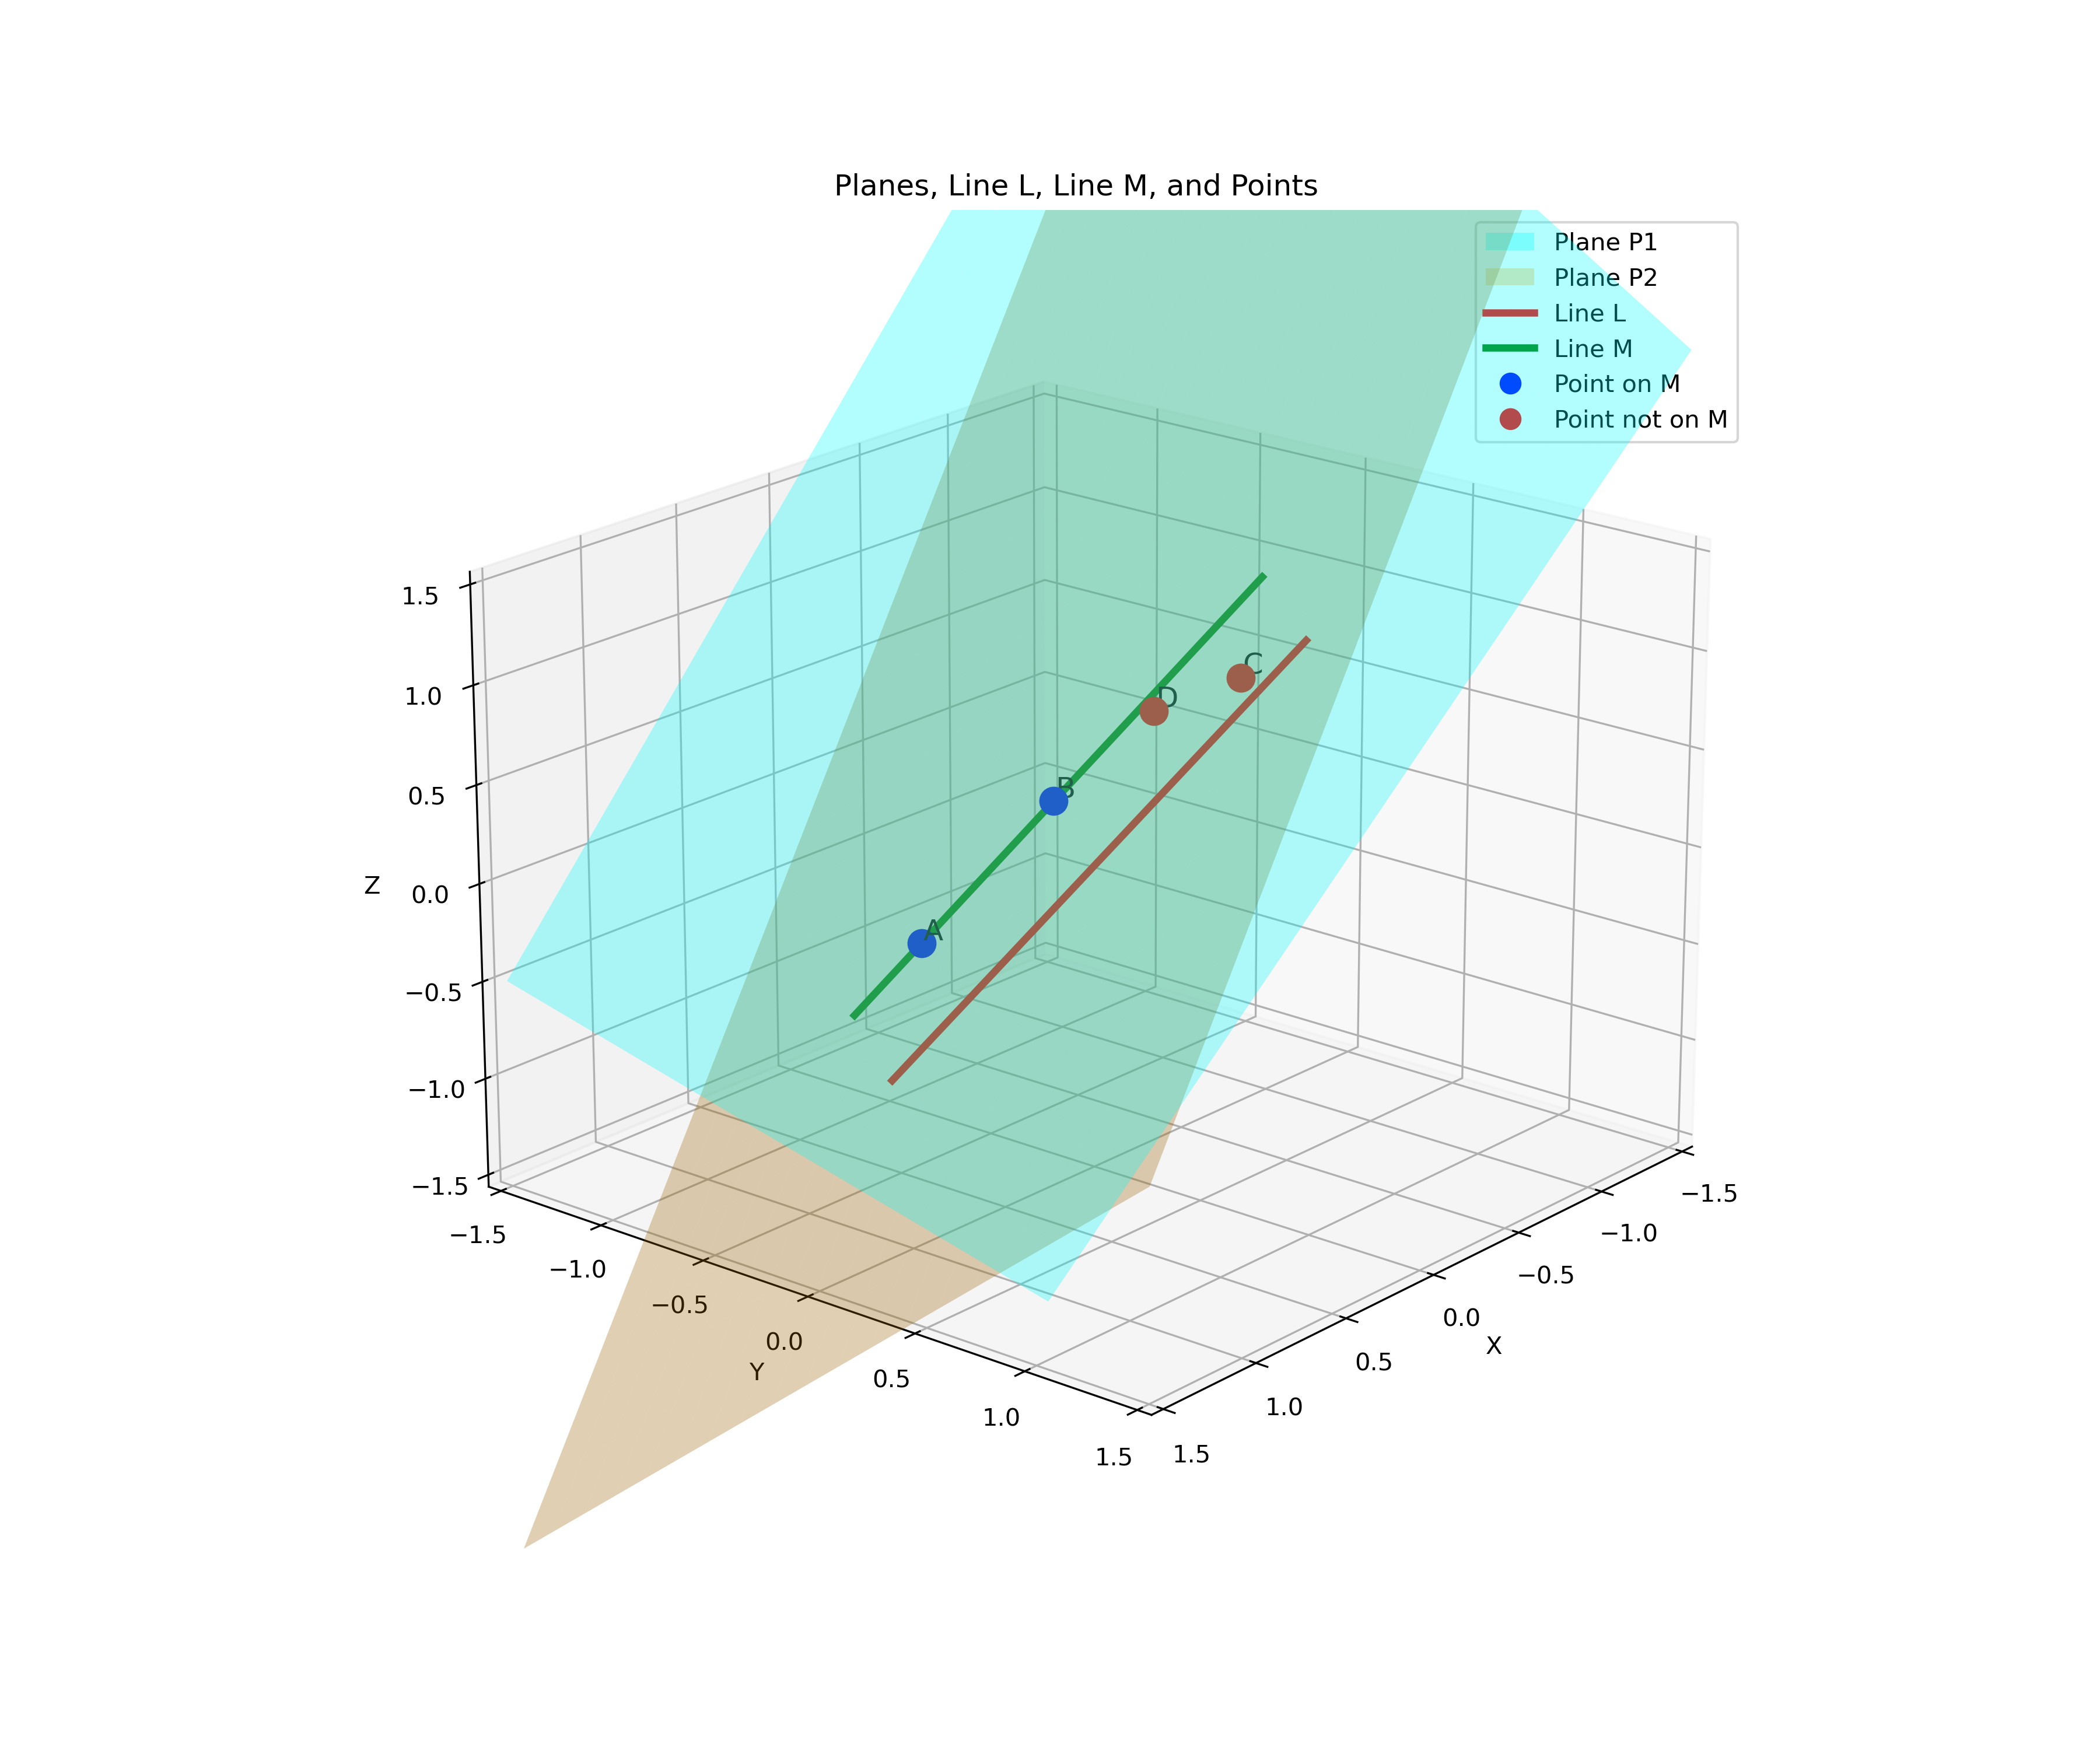
\includegraphics[width=\columnwidth, height=0.8\textheight, keepaspectratio]{../figs/planes_lines_points_ctypes.png}     
\end{frame}

	


\end{document}


